\chapter{Methode} % Main chapter title
\label{chapter3:Methode} % Change X to a consecutive number; for referencing this chapter elsewhere, use \ref{ChapterX}

\section{Design eigener Sniffer}
\label{Design Sniffer}

Zu Beginn der Projektarbeit wurde ein Prozessdiagramm erstellt, welches aufzeigen soll, welche Hardware benötigt wird um einen Sniffer zu entwickeln, welcher vom MVB lesen kann.
Dieser erste Entwurf ist in Abbildung \ref{fig:AufbauSnifferDraft} zu sehen.

\begin{figure}[H]
    \centering
    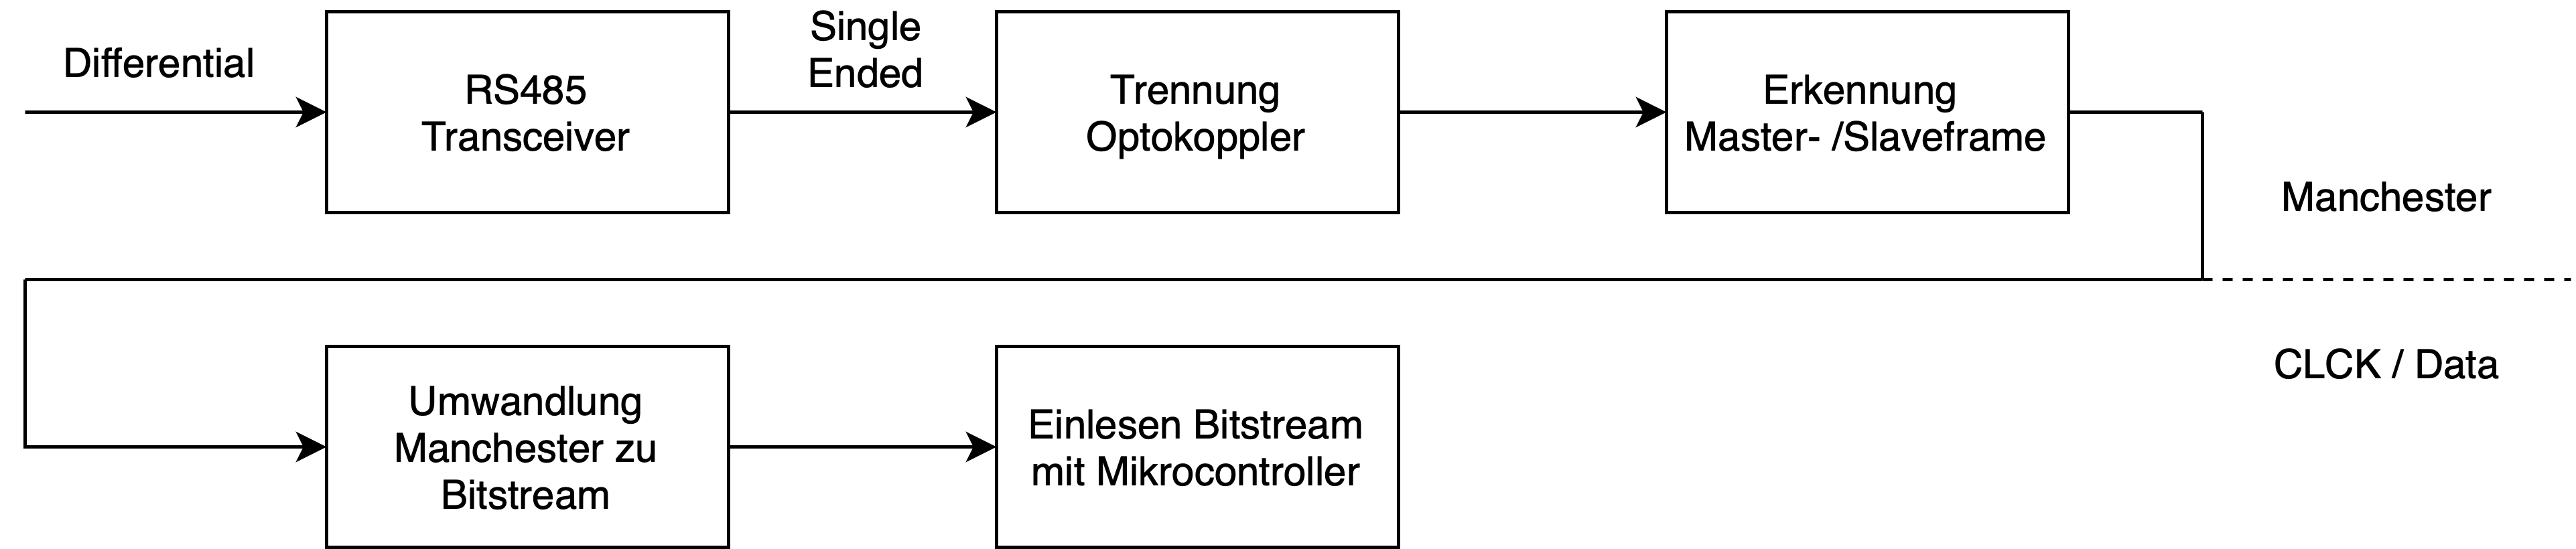
\includegraphics[width=1\linewidth]{Figures/Chap3/Design Eigener Sniffer/Draft_Aufbau_Sniffer.png}
    \caption{Erste Darstellung Aufbau Sniffer}
    \label{fig:AufbauSnifferDraft}
\end{figure}

Der Entwurf diente als Grundlage auf welcher aufgebaut werden konnte. Aus dem Entwurf entstand dann
ein ausführlicher schematischer Aufbau, in dem auch gleich die Anforderungen zum Sniffer aufgeführt
sind. 

Dieser Aufbau, wie er in Abbildung \ref{fig:AufbauSniffer} zu sehen ist, zeigt die verwendete Hardware
auf und wie diese untereinander verbunden sind.

\begin{figure}[H]
    \centering
    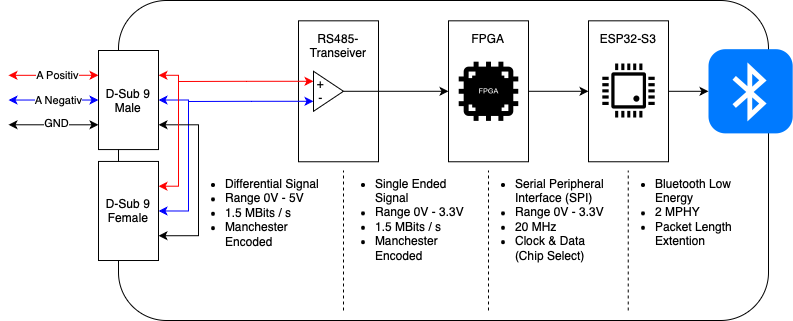
\includegraphics[width=0.9\linewidth]{Figures/Chap3/Design Eigener Sniffer/Aufbau_Sniffer.png}
    \caption{Schematischer Aufbau Sniffer}
    \label{fig:AufbauSniffer}
\end{figure}


Es ist zu sehen dass vom ersten zum finalen Aufbau, der Baustein "'\textit{Trennung Optokoppler}"'
wegfällt, da durch den RS485-Transceiver sichergestellt wird, dass der Bus nie beschrieben werden kann.
Im finalen Design kommt zusätzlich die Ausgabe über Bluetooth hinzu welche zu beginn nicht angedacht
war.

Um aus dem differentiellen Manchestersignal vom MVB ein Single-Ended Signal, welches "'0 V"' bei einer 
negativen Flanke und "'3.3 V"' bei einer positiven Flanke annehmen soll, erzeugen zu können, wurde ein
RS485-Transceiver verwendet. Der Transceiver wird mit einer Spannung von "'3.3 V"' versorgt. Das
erzeugte digitale Signal vom RS485 wird weiter ins Field Programmable Gate Array (FPGA) geleitet, wo
der Manchestercode decodiert wird und als Bitstream über das SPI an den Mikrocontroller ESP32 gesendet
wird. Der Mikrocontroller wertet die Daten aus und gibt dann die entsprechenden Codes per Bluetooth aus.

In einer Prototypenphase und somit auch im Rahmen der Projektarbeit, sind dafür drei verschiedene
Evaluationsboards verwendet worden. Das definierte Ziel für den fertigen Sniffer, welches in der
Bachelorarbeit angestrebt wird, ist es ein eigenes PCB zu erstellen, welche die benötigten Bauteile auf
einem Board vereint. Ebenfalls soll der fertige Sniffer ein schützendes und abschliessendes Gehäuse,
mit den nötigen Ausschnitten besitzen.

\subsection{Wahl der Hardware}
In den folgenden Kapitel wird erläutert warum die entsprechende Hardware für den MVB-Sniffer gewählt
wurde. In den Kapitel \ref{chapter5:Diskussion} und \ref{chapter6:Ausblick} werden die Wahl der
Hardware nochmals abschliessend diskutiert und, allfällige Änderungen in der Wahl, als Ausblick 
festgehalten.


\subsubsection{RS485}
Der RS485 Transceiver macht aus einem differentiellen Signal ein digitales Signal, welches zwischen der Speisespannung und 0V hin und her wechselt. Das Ausgangssignal kann im Falle des MVB von Busteilnehmern ausgewertet werden. Da im Anwendungsbereich des MVB (ESD) auf den Schienenfahrzeugen, für welche der Sniffer ausgelegt wird, bereits RS485 Transceiver eingesetzt werden, war es naheliegend und sinnvoll diese auch für den Sniffer einzusetzen.

\subsubsection{FPGA}
In einer ersten Recherche war eine Lösungsvariante, die Decodierung des Manchestersignal in einer reinen Hardwarelösung wie sie in Abbildung \ref{fig:Manchester Decoder} zu sehen ist umzusetzen.

\begin{figure}[H]
    \centering
    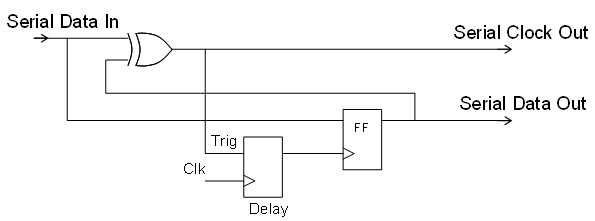
\includegraphics[width=0.6\linewidth]{Figures/Chap3/Design Eigener Sniffer/manchester_decoder.png}
    \caption{Manchester Decoder \cite{Manchester_Decoding}}
    \label{fig:Manchester Decoder}
\end{figure}
%\textcolor{red}{Bild von https://community.infineon.com/t5/PSOC-5-3-1/Machester-Decoder-using-Psoc/td-p/41723}

Als eine weitere Variante wurde das FPGA zur Umsetzung des Decoders in Betracht gezogen.
Der Entscheid für den FPGA und gegen die nicht programmierbare, reine Hardwarelogik lag in folgenden Punkten:
\begin{itemize}
  \item Die Logik des FPGA ist flexibel und schnell anpassbar.
  \item Das FPGA kann weiter konfiguriert werden und bei einer Weiterentwicklung des Sniffers können weitere Aufgaben problemlos implementiert werden.
  \item Das Interesse ein FPGA und dessen Programmierung in Very High-Speed Integrated Circuit Hardware Description Language (VHDL) näher kennen zu lernen war gross und in diesem Projekt gut realisierbar.
\end{itemize}

Für die Projektarbeit wurde das FPGA-Entwicklungskit 10M08SAE144C8G zur Verfügung gestellt.

\subsubsection{SPI}
Für die Kommunikation zwischen FPGA und ESP32 wurde das Protokoll SPI gewählt, weil es diese Kommunikation möglich macht gleichzeitig zu schreiben, sowie Daten zu empfangen (Full Duplex fähig). Des Weiteren können mit diesem Übertragungsprotokoll sehr hohe Raten erreicht werden, welche bei der berechneten Busauslastung (siehe Kapitel \ref{fig:MessaufbauBusauslastungMessen}) von Vorteil ist. Alternativ hätten weitere Protokolle gewählt werden können. In Tabelle \ref{tab:spi_vergleich} ist ein kurzer Vergleich von SPI und zwei alternativen Kommunikationsprotokollen (I²C und UART) zu sehen. SPI ist dabei, wie bereits erwähnt, mit Abstand am schnellsten und einfach zu implementieren. \cite{SPI}

\begin{table}[ht]
\renewcommand{\arraystretch}{1.5} % Zeilenabstand erhöhen
\centering
\begin{tabular}{@{}p{3.4cm}p{3.2cm}p{3.2cm}p{3.2cm}@{}}
\toprule
\textbf{Merkmal}        & \textbf{SPI} & \textbf{I²C} & \textbf{UART} \\ \midrule
\textbf{Kommunikationsart} & Full duplex & Half duplex & Half duplex \\
\textbf{Anzahl Leitungen} & 4 (MISO, MOSI, SCLK, SS) & 2 (SDA, SCL) & 2 (TX, RX) \\
\textbf{Taktung}        & Synchron & Synchron & Asynchron \\
\textbf{Datenrate}      & 50+ MBit/s & Bis zu 4 MBit/s & Bis zu 1 MBit/s \\
\textbf{Vorteile}       & Hohe Datenrate, Full duplex, einfache Hardware & Wenige Leitungen, mehrere Geräte auf einem Bus & Einfach zu implementieren, universell einsetzbar \\
\textbf{Nachteile}      & Viele Leitungen bei mehreren Slaves, keine eingebaute Fehlerkorrektur & Geringere Geschwindigkeit, zusätzliche Protokollverwaltung & Keine Taktleitung, potenziell ungenau bei Baudrate-Mismatch \\
\bottomrule
\end{tabular}
\caption{Vergleich zwischen SPI, I²C und UART}
\label{tab:spi_vergleich}
\end{table}

\subsubsection{ESP32}
Der ESP32 wurde gewählt, weil bereits Erfahrungen im Programmieren des IoT Chips in der Gruppe vorhanden sind und die ESP32 Familie die nötigen Peripherie-Elemente wie SPI und Bluetooth Low Energy bereits implementiert hat. Die S3 Variante wurde spezifisch gewählt, da es ein Dual-Code Prozessor ist und ein USB-OTG Controller implementiert ist, welcher das direkte Schreiben auf USB-Sticks ermöglicht. 

